\documentclass[11.5pt]{article}
\usepackage[margin=1in]{geometry}
\usepackage{hyperref}
\usepackage{algorithm}% http://ctan.org/pkg/algorithms
\usepackage{algpseudocode}% http://ctan.org/pkg/algorithmicx
\usepackage{graphicx}
\usepackage{caption}
\usepackage{subcaption}
\usepackage{tikz}
\def\checkmark{\tikz\fill[scale=0.4](0,.35) -- (.25,0) -- (1,.7) -- (.25,.15) -- cycle;}

\title{Stance Detection for the Fake News Challenge Dataset using Deep Learning}

\author{Anak Agung Ngurah Bagus Trihatmaja and Shishir Kurhade}

\date{}

\begin{document}

\maketitle

\abstract
The problem of fake news has arisen recently as a threat to high-quality 
journalism and well-informed public disclosure. The goal of fake news 
challenge is to explore how artificial intelligence technologies, particularly
machine learning and natural language processing, might be leveraged to combat 
the fake news problem\cite{fake_news_challenge}. The goal of our project is to develop machine learning 
models to predict a stance label (‘Agrees’, ’Disagrees’, ’Related’, ’Unrelated’) 
with respect to the title for a respective news article. For this purpose, we 
will use the gated recurrent unit (GRU) to predict the labels. As a baseline to 
measure performance we will also solve the problem using logistic regression method.

\vspace{2mm}
\section{Introduction}
In this project, we try to combat a serious problem in our media using machine 
learning techniques. In a poll conducted by Pew Research Center, 64\% of US 
adults said that fake news has caused a “great deal of confusion” about the 
basic facts of current issues and events\cite{barthel_mitchell_holcomb_2016}. 
This problem views the task of fake-news detection as a stance detection problem 
which is a labeling task. We want to automatically classify a news into four labels, 
which are ‘unrelated’, ‘agrees’, ‘disagrees’, and ‘discusses’.  

A reasoning for these labels is as follows:
\begin{enumerate}
  \item \textbf{Agrees}: The body text agrees with the headline.
  \item \textbf{Disagrees}: The body text disagrees with the headline.
  \item \textbf{Discusses}: The body text discuss the same topic as the headline, 
    but does not take a position
  \item \textbf{Unrelated}: The body text discusses a different topic than the headline
\end{enumerate}

The classifier that we build could later be used as a base of a 
fake news detection tool that can automatically categorize the news into the 
stances given.

\section{Technical Approach}

Our problem of stance detection can be viewed as that of text classification with each of the stances as a possible class. We use two approaches to solve this problem viz. logistic regression and deep neural networks.

\subsection{Logistic Regression}

Logistic is the appropriate regression analysis to conduct when the dependent variable is dichotomous (binary). Logistic regression is used to describe data and to explain the relationship between one dependent binary variable (stances in our case) and one or more independent variables (words in the vocabulary). 
In our problem setting we aim at classifying every news article body in a stance with respect to the title. For representing the text as features we use a representation form called tf-idf (term frequency – inverse document frequency) matrix. Here, each document is represented as a vector with respect to the vocabulary of words. The model concatenates the text from the title and the body of an news article to prepare a vectorised representation. This representation increases the values of weights for words proportionally to the number of times a word appears in the document and is offset by the frequency of the word in the corpus. This is helpful in our task as the news articles are of variable length, thus giving us a robust feature representation. We perform ‘one vs all’ regression for each stance. 
In pseudocode, the training algorithm for an One vs All learner constructed from a binary classification learner L is as follows:

\begin{algorithm}[H]
  \caption{Logistic regression}\label{logistic}
  \textbf{Input}

  \hspace*{\algorithmicindent}L (training algorithm for binary classifiers)

  \hspace*{\algorithmicindent}samples $X$

  \hspace*{\algorithmicindent}labels $y$ where $y_i \in \{1, ..., K\}$ is the label for the sample $X_i$ 

  \textbf{Output}

  \hspace*{\algorithmicindent}a list of classifiers $f_k$ for $k \in \{1, ..., K\}$

  \begin{algorithmic}[1]
    \Procedure{LogisticRegression}{}
    \For{$k\gets 1, K$}
    \If{$y_i = k$}
    \State $z_i \gets 1$
    \Else
    \State $z_i \gets 0$
    \EndIf

    \State $f_k\gets L(X, z)$\Comment{Apply $L$ to $X$, $z$ to obtain $f_k$}
    \EndFor
    \EndProcedure
  \end{algorithmic}
\end{algorithm}

Making decisions means applying all classifiers to an unseen sample $x$ and predicting the label $k$ for which 
the corresponding classifier reports the highest confidence score $f_k$.
 
\subsection{Deep Neural Networks}

Neural networks are a set of algorithms, modelled loosely after the human brain, that are designed to recognize patterns. They interpret sensory data through a kind of machine perception, labeling or clustering raw input. The patterns they recognize are numerical, contained in vectors, into which all real-world data, be it images, sound, text or time series, must be translated. 
Traditionally RNNs have been widely used in NLP tasks because of their memory capabilities helping them to retain the sequence information in the text, thus developing better language models. However, they suffer from problems of vanishing gradient and variants of RNNs consisting of LSTM and GRU cells solve this problem. As GRUs are faster and computationally less expensive we implemented our network using GRU cells in Tensorflow to predict the stances. For feature representation we embed each word in the title and article body using GloVe representations into vectors of size 50. These are pre-trained word vector representations made readily available by Stanford NLP group. We have tried two variants of neural networks for our task:

\begin{enumerate}
  \item Vanilla RNN with single hidden layer   
  \item RNN with multiple hidden layers and dropout  
\end{enumerate}

The input layer consisting of 50 GRU cells accepts one word at a time from the input news 
title and article whose output is then used as an input for the next hidden layer. 
This pipelining of outputs as input to next layer continues for all hidden layers and 
the final layer which consists of softmax layer classifies the stance. 
We use the cross entropy loss function to calculate the loss and optimize it using the Adam Optimizer.
 It is important to note that the neural network preserves the sequential information present in the sentences 
to generate weights for classifying the test samples unlike the baseline method which is a bag of words model. 

\section{Experimental Results}

\subsection{Dataset Overview}

The data provided by the Fake News Challenge consists of 
headline, body, and stace. 
For training, there are two csv files:
\begin{enumerate}
  \item \textit{train\_bodies.csv}: contains the body text of articles with its ID
  \item \textit{train\_stances.csv}: contains labeled stances for pairs of article 
      headlines and article bodies, in which the article bodies refer to the 
      bodies in train\_bodies.csv
\end{enumerate}

The distribution of the data is as follows:
\begin{table}[h]
  \centering
  \begin{tabular} 
    {|c|c|c|c|c|}
    \hline
    Rows & Unrelated & Discuss & Agree & Disagree \\
    \hline
    49972 & 0.73131 & 0.17828 & 0.0736012 & 0.0168094 \\
    \hline
  \end{tabular}
  \caption{Dataset distribution}
\end{table}

We will roughly use 4000 samples as our development set, for choosing 
hyperparameter and performance evaluation, and use the rest for training. Meanwhile, for the test dataset we use 4000 samples for testing our model.

\subsection{Data Pre-processing}

For both logistic and RNN, we will do the same data cleaning procedures. There is a difference in feature representation for each of the models.
The data cleaning procedures we perform is as follows:

\begin{enumerate}
  \item Normalize the case
  \item Remove all punctuations and non-alphabetic symbols 
  \item Replace the shorten words with the normal words, for example: you'll into you will
\end{enumerate}

 
In case of logistic regression to reduce dimentionality, we perform lemmatization on the text generated from concatinating headlines and the bodies. 
We then build our tf-idf matrix with this vocabulary and data using scikit-learn \cite{scikit-learn}. The tf-idf matrix looks like below.

\begin{table}[h]
  \centering
  \begin{tabular} 
    {|c|c|c|c|c|c|}
    \hline
    & Word 1 & Word 2 & Word 3 & Word 4 & ... \\
    \hline
    Document 1 & 0.01 & 0.0 & 0.05 & 0.13 & 0.12 \\
    \hline
    Document 2 & 0.2 & 0.0 & 0.04 & 0.4 & 0.1 \\
    \hline
    Document 3  & 0.12 & 0.0 & 0.101 & 0.012 & 0.0 \\
    \hline
  \end{tabular}
  \caption{Input representation for logistic regression}
\end{table}

Each row in the table represents one document we have in the dataset. While, each column represents a word present in the vocabulary.

For RNN using GRUs, we represents our data as word vectors. The text from the corpus will be mapped to corresponding vectorized
forms using  pre-trained \textit{GloVe} 
representations--freely available on the Stanford NLP group website\cite{Bird:2009:NLP:1717171,pennington2014glove}. 
Since the text sequences observed will be of variable length we will pad all 
sequences to the length of the maximum length text sequence before inputting 
it to our model. The representation of the matrix can be seen as follows-

\begin{table}[h]
  \centering
  \begin{tabular} 
    {|c|c|c|}
    \hline
    & Headlines & Bodies \\
    \hline
    Document 1 & [0.23, 0.12, ...], [0.123, 0.14, ...], ... & [0.05, 0.012, ...], [0.121, 0.123, ...] \\
    \hline
    Document 2 & [0.23, 0.12, ...], [0.119, 0.4, ...], ... & [0.11, 0.011, ...], [0.109, 0.89, ...] \\
    \hline
    Document 3 & [0.28, 0.1, ...], [0.134, 0.3, ...], ... & [0.05, 0.001, ...], [0.121, 0.189, ...] \\
    \hline
  \end{tabular}
  \caption{Input representation for neural network}
\end{table}

As our training dataset is skewed and has a majority of stances as 'unrelated', we separate our training dataset into two. The first dataset contains related vs related stances where (agree, disagree, discuss) are together bucketed into 'related'. The second is a dataset containing only agree, disagree, discuss. We then train our models separately for each dataset.

In the case of RNNs, we represent the label as a vector. For the unrelated and related stance, we represent it as $[1, 0]$ if it is unrelated and $[0, 1]$ as related.
While, for the second dataset we label our dataset as $[1, 0, 0]$ if the stance is agree, $[0, 1, 0]$ if the stance is disagree and $[0, 0, 1]$ as discuss. The final structure of our data for RNN looks as follows.

\begin{table}[h]
  \centering
  \begin{tabular} 
    {|c|c|c|c|}
    \hline
    & Headlines & Bodies & Stances \\
    \hline
    Document 1 & [0.23, 0.12, ...], [0.123, 0.14, ...], ... & [0.05, 0.012, ...], [0.121, 0.123, ...] & [0,1] \\
    \hline
    Document 2 & [0.23, 0.12, ...], [0.119, 0.4, ...], ... & [0.11, 0.011, ...], [0.109, 0.89, ...] & [1, 0] \\
    \hline
    Document 3 & [0.28, 0.1, ...], [0.134, 0.3, ...], ... & [0.05, 0.001, ...], [0.121, 0.189, ...] & [1,0] \\
    \hline
  \end{tabular}
  \caption{Final input representation for neural network}
\end{table}

\subsection{Experimental Settings}

Our dataset consists of 4 classes (unrelated, agrees, disagrees, discuss) with headline and body as features for the RNNs. Each word in GRU is represented as a vector of length 50.
For the logistic regression, we have 33795 unique and lemmatized words used as features represented in form of tf-idf matrix.

We train our models on a computer with Intel i7-8550U CPU @ 1.80GHz × 8 and 16 GB of RAM. The neural network takes four hours to train while the logistic regression model takes about ten minutes
For getting the test result, we run our test for the neural network on AWS (Amazon Web Services) EC2 p3.2xlarge package running Ubuntu with specifications as-

\begin{table}[h]
  \centering
  \begin{tabular} 
    {|c|c|c|c|}
    \hline
    GPUs - Tesla V100 & GPU Memory (GB) & vCPUs & Memory (GB) \\
    \hline
    1 & 16 & 8 & 61 \\
    \hline
  \end{tabular}
  \caption{AWS specification}
\end{table}

\subsection{Validation}

We get the best value for regularization using cross validation on our logistic regression model. We run the the logistic with several C values. The C in denotes the inverse of regularization strength. The results of the cross validation are as follows-

\begin{figure}[h!]
  \begin{subfigure}{.5\textwidth}
    \centering
    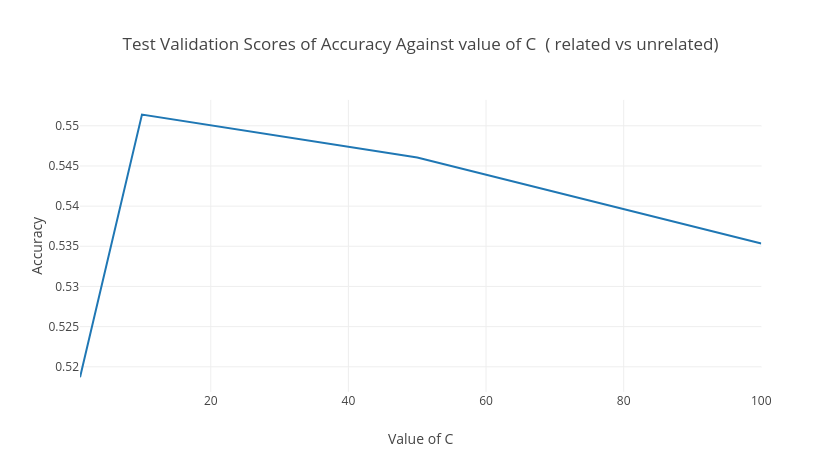
\includegraphics[width=.9\linewidth]{plot_1}
  \end{subfigure}
  \begin{subfigure}{.5\textwidth}
    \centering
    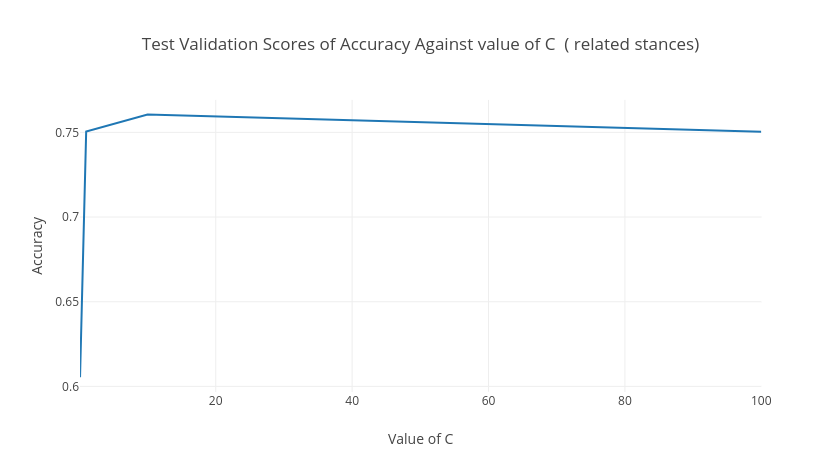
\includegraphics[width=.9\linewidth]{plot_2}
  \end{subfigure}
  \caption{Test validation scores against value of C for each dataset}
  \label{fig:logistic}
\end{figure}

\begin{table}[h!]
  \centering
  \begin{tabular} 
    {|c|c|c|c|}
    \hline
     & C = 1e-15 & C = 1 & C = 1000 \\
    \hline
    Agree & 0 \% & 71 \% & 68 \% \\
    \hline
    Disagree & 0 \% & 0 \% & 46 \% \\
    \hline
    Discuss & 59 \% & 77 \% & 79 \% \\
    \hline
  \end{tabular}
  \subcaption{Precision score for different value of C in related stances dataset}
  \begin{tabular} 
    {|c|c|c|c|}
    \hline
     & C = 1e-15 & C = 1 & C = 1000 \\
    \hline
    Agree & 0 \% & 63 \% & 66 \% \\
    \hline
    Disagree & 0 \% & 0 \% & 19 \% \\
    \hline
    Discuss & 100 \% & 89 \% & 85 \% \\
    \hline
  \end{tabular}
  \subcaption{Recall score for different value of C in related stances dataset}
\end{table}

For the GRU, we run the validation using different number of neurons. We then pick the best result.

\begin{figure}[h!]
  \begin{subfigure}{.5\textwidth}
    \centering
    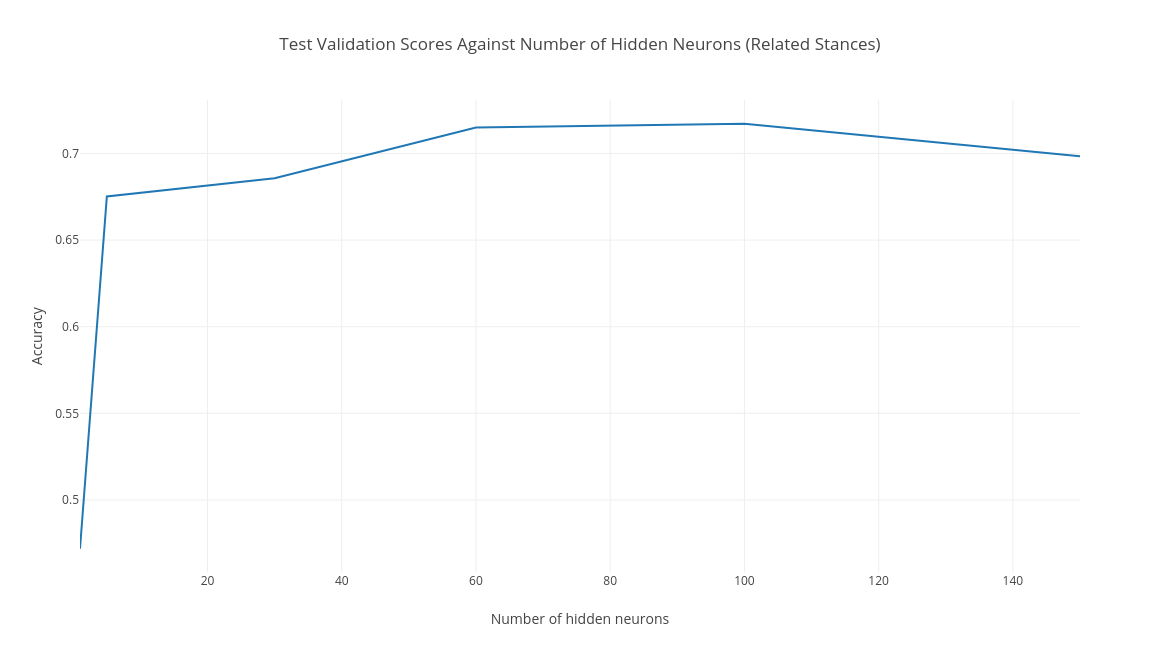
\includegraphics[width=.9\linewidth]{plot_9}
  \end{subfigure}
  \begin{subfigure}{.5\textwidth}
    \centering
    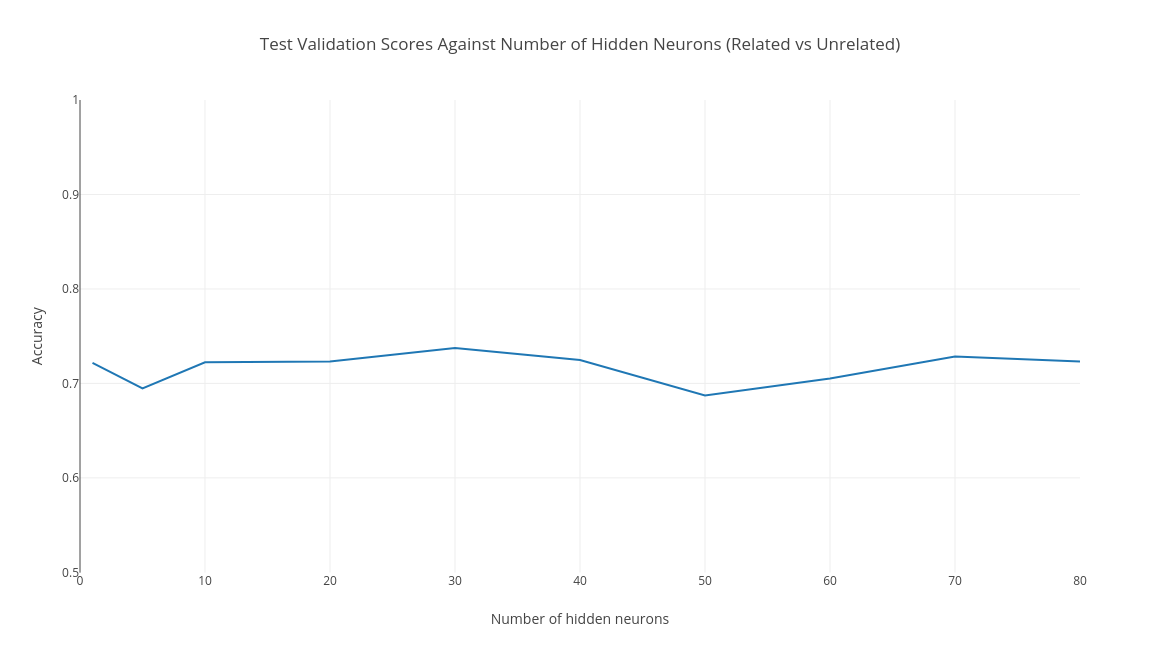
\includegraphics[width=.9\linewidth]{plot_11}
  \end{subfigure}
  \caption{Test validation scores against number of hidden neurons for each dataset}
  \label{fig:neurons}
\end{figure}

The graph above shows the effect of number of neurons in a layer for each dataset. We can see that the accuracy reaches its peak when there are 60 neurons in hidden layer for unrelated vs related dataset, while for the related stances
the accuracy is quite similar for every number of neurons. Therefore we choose 60 as the number of neurons in the hidden layers.

\subsection{Results and Analysis}

\begin{table}[h]
  \centering
  \begin{tabular} 
    {|c|c|c|c|}
    \hline
    Accuracy & Logistic regression & RNN with 1 hidden layer & RNN with 2 hidden layers \\
    \hline
    Related vs unrelated & 52.76 \% & 81.58 \% & 78.66 \% \\
    \hline
    Related stances & 66.03 \% & 56.94 \% & 61.19 \% \\
    \hline
  \end{tabular}
  \caption{Results from RNN and logistic regression}
\end{table}

We also calculated the accuracies for three hidden layers in RNN and the accuracy for related stances dropped drastically to 21.2 \%.
For related vs unrelated stances (agree, disagree, discuss together form unrelated) we use the entire dataset while training and for the related stances training we only use agree, disagree,
discuss stances which form around 27 \% of the total training data. Logistic regression performs better on smaller datasets and hence has high accuracy for related stances. The neural networks give a good performance when there is a large dataset available to train them. This explains their higher accuracy as compared to logistic regression for related vs unrelated stances. Considering the overall performances of the models we conclude that a RNN model with two hidden layers is best suitable for our problem.

\section{Participants Contribution}

\begin{table}[h]
  \centering
  \begin{tabular} 
    {|c|c|c|}
    \hline
    \textbf{Tasks} & \textbf{Trihatmaja} & \textbf{Kurhade} \\
    \hline
    Data pre-processing for logistic regression & & \checkmark \\
    \hline
    Data pre-processing for RNN & \checkmark & \\
    \hline
    RNN implementation & \checkmark & \\
    \hline
    Logistic regression implementation & & \checkmark \\
    \hline
    Server environment setup & \checkmark & \\
    \hline
    RNN improvement & & \checkmark \\
    \hline
    Logistic regression cross validation & \checkmark & \\
    \hline
    RNN test & & \checkmark \\
    \hline
    Presentation, project proposal and report & \checkmark & \checkmark \\
    \hline
  \end{tabular}
\end{table}

\vspace{10mm}

\bibliographystyle{unsrt}
\bibliography{2380985}
\end{document}
